\documentclass[english,12pt,a4paper]{article}

%%%%%%%%%%%%%%%%%%%%%%%%% packages %%%%%%%%%%%%%%%%%%%%%%%%
\usepackage{amsmath}
\usepackage{amssymb}
\usepackage{mathrsfs}
\usepackage{amsthm}
\usepackage{amsfonts}
\usepackage{graphicx}
\usepackage[T1]{fontenc}
\usepackage[latin9]{inputenc}
\usepackage{textcomp}
\usepackage{listings}
\usepackage[all]{xy}
\usepackage{verbatim}
\usepackage[left=2cm,right=2cm,top=3cm,bottom=2.5cm]{geometry}
\usepackage{float}

%%%%%%%%%%%%%%%%%%%%% students data %%%%%%%%%%%%%%%%%%%%%%%%
\newcommand{\student}{NONO SAHA Cyrille Merleau}
\newcommand{\course}{Essay 2018}
\newcommand{\assignment}{Assignment I } 
%%%%%%%%%%%%%%%%%%% using theorem style %%%%%%%%%%%%%%%%%%%%
\theoremstyle{definition}
\newtheorem{theorem}{Theorem}
\newtheorem{lemma}[theorem]{Lemma}
\newtheorem{definition}[theorem]{Definition}
\newtheorem{example}[theorem]{Example}
\newtheorem{remark}[theorem]{Remark}
\newtheorem{corollary}[theorem]{Corollary}
\makeatletter
\usepackage{listings}
\usepackage{color}

\definecolor{dkgreen}{rgb}{0,0.6,0}
\definecolor{gray}{rgb}{0.5,0.5,0.5}
\definecolor{mauve}{rgb}{0.58,0,0.82}


%%%%%%%%%%%%%%%%%%%%%%%%%%%%%% LyX specific LaTeX commands.
\newcommand{\lyxmathsym}[1]{\ifmmode\begingroup\def\b@ld{bold}
  \text{\ifx\math@version\b@ld\bfseries\fi#1}\endgroup\else#1\fi}


\makeatother

\usepackage{babel}
\begin{document}
1. $P=5.99738735870816+1.29466289806164e19*T^{9}+7.34641531797667\times10^{-12}/T^{4}-1759.61951015184*T-139404.24651719*T^{2}$

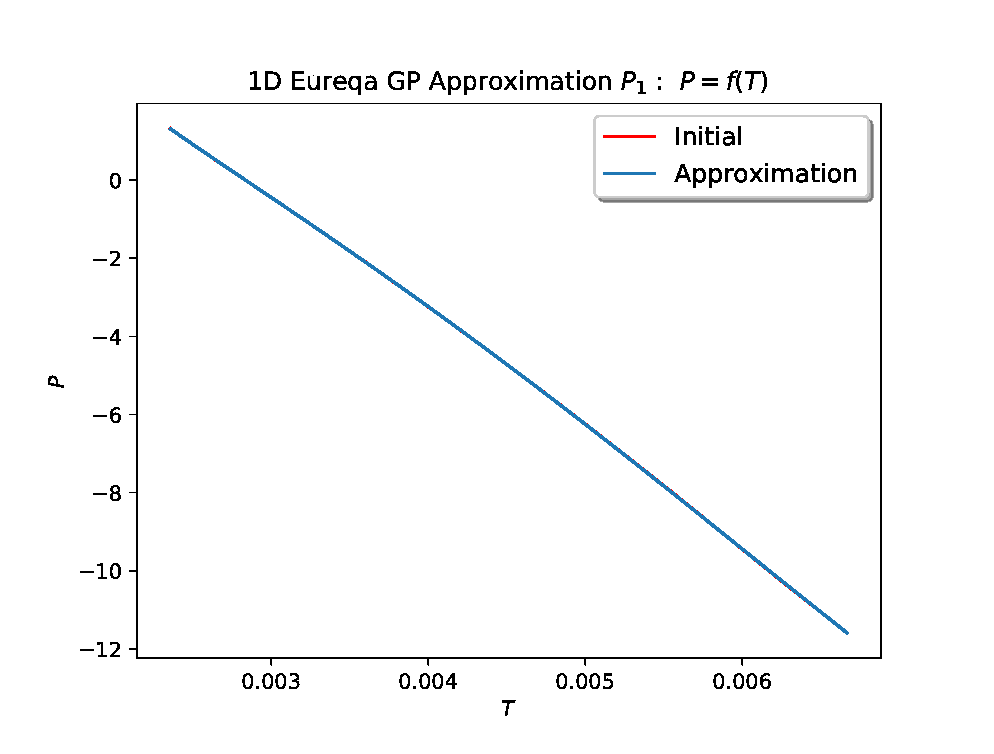
\includegraphics[scale=0.7]{Test1DEqP1}

\vspace{0.5cm}

2. $P=6.9077421887099-2169.089730967*T-13968.0187918922*T^{3}-92338.7237579469*T^{2}$

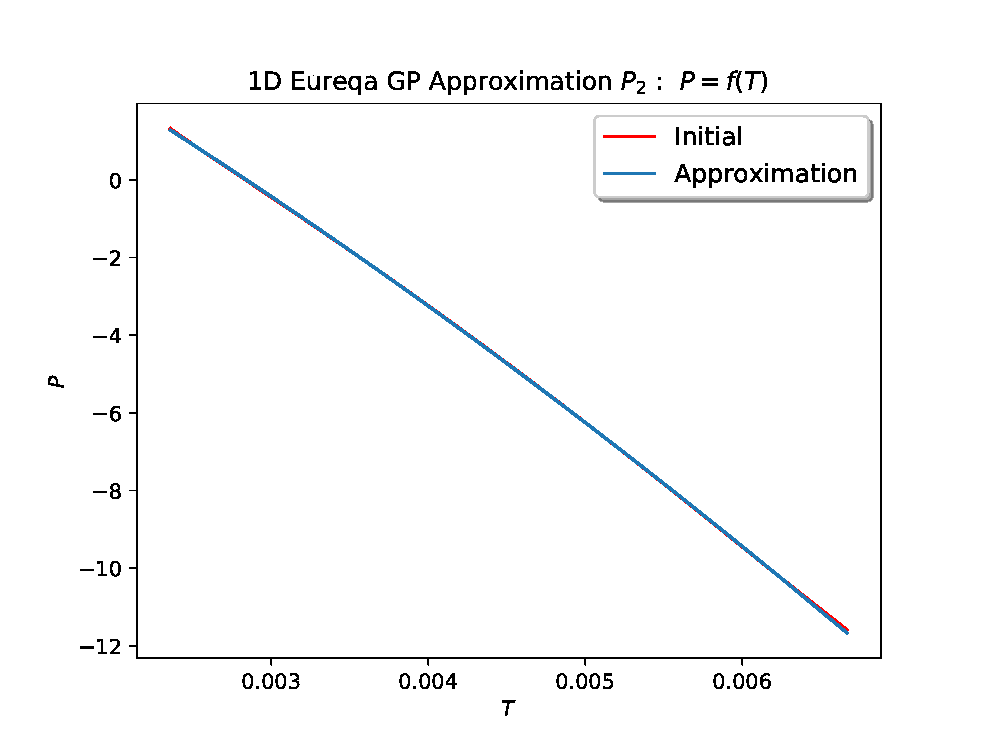
\includegraphics[scale=0.7]{Test1DEqP2}

\newpage{}

3. $P=6.95897107874203-2194.59122457971*T-89338.80860464*T^{2}$

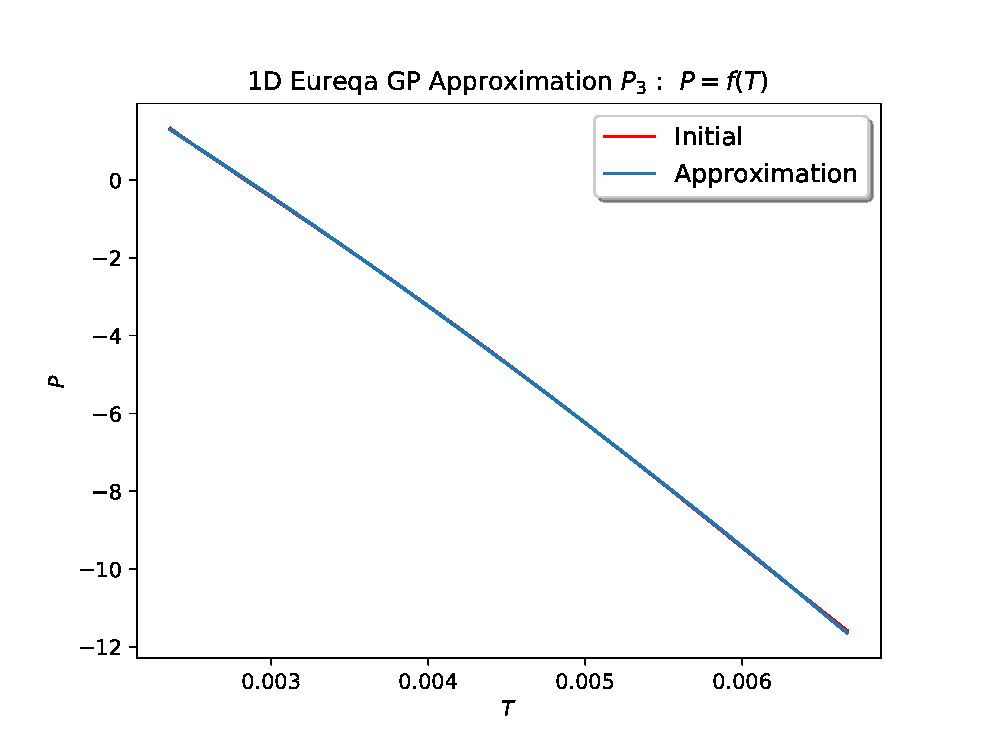
\includegraphics[scale=0.7]{Test1DEqP3}

\vspace{0.5cm}

4. $P=8.1603154015448\text{\textendash}2881.13073910938*T$


\end{document}
